\chapter{序論}
\section{研究の背景と目的}
近年,AI分野は急速な発展を続けているh.
%第1次AIブームについて述べる
第一次ブームはコンピュータができ始めた1950~60年代です。コンピュータの登場により人間を超えるようなAIが誕生すると期待され、次々と新しいアルゴリズムが考案されました。第一次ブームの特徴として「推論と探索」があります。「推論と探索」とはコンピュータがゲームやパズルを解いたり、迷路のゴールへの生き方を調べるなどの技術のことです。第一次ブームの研究により生み出された新しいアルゴリズムにより、一見知的な活動を行えるようになりましたが、コンピュータの性能は低く、ルールとゴールが厳密に決まっている枠組のなかでしか動けないため、現実世界では全く役に立たないことが見えてきました。その結果、第一次AIブームは終結してしまいます。これらの第一次ブームでの人工知能のことをトイプロブレム(おもちゃの問題)と呼ばれます。コンピュータの性能の限界が見えたことから、1970年代に一回目の冬の時代に突入していきます.\\
%第2次AIブームについて述べる
1980年代に入り、家庭にコンピュータが普及したことにより第二次ブームが発生しました。第二次AIブームの特徴として「エキスパートシステム」が挙げられます。「エキスパートシステム」とは専門家の知識をコンピュータに教え込みことで現実の複雑な問題を人工知能に解かせることを試みたシステムです。第一次ブームと比較してコンピューターの小型化・性能が高まっており、ある程度はこれらの試みは成功しましたが、知識を教え込む作業が非常に煩雑であること、例外処理や矛盾したルールに柔軟に対応することが出来ませんでした。日常世界を見渡してみると、これらの例外処理や矛盾したルールは非常に多く、知識を教え込む作業が非常に困難なことから、第二次AIブームは自然に消滅へと向かってしまいました。その後、1990年代半ばにWindows95の登場、インターネットの普及、検索エンジンの高性能化が進み、世界中にいる誰もが簡単に大量のデータを扱える時代に突入しました.\\
%第3次AIブームについて述べる
第二次AIブームでのエキスパートシステムが壁にぶつかった問題として、日常世界には例外処理や矛盾したルールが非常に多く、知識を教え込む作業が非常に困難というのがありました。これはコンピュータはプログラムと呼ばれるあらかじめINPUTされた命令を順次行っていくため、INPUTされていない例外処理や、矛盾したルールにぶち当たった場合に柔軟に対応出来なかったためです。これらを解決する手段として「機械学習」や「ディープラーニング」にてコンピュータが自らが学んでいくという手法が第二次AIブームの時代から研究されていましたが、実用化するためにはコンピュータの性能が追い付いていませんでした。しかし、2000年代に入り、コンピューターの小型化・性能向上に加えインターネットの普及、クラウドでの膨大なデータ管理が容易となったことで実現可能なレベルとなり、第三次AIブームが沸き起こりました。第三次AIブームでの主な出来事1997年:チェス専用のコンピューターが世界王者に勝利2006年:ディープラーニングの実用方法が登場2011年:IBMワトソンがクイズ番組で人間に勝利する2012年:画像認識の向上で画像データから「猫」を特定できるようになる2016年:「アルファ碁」がプロ棋士に勝利を収める2016年はディープラーニングを起爆剤としたAIが社会に衝撃を与え急速に発達した年であると言われています。次の年の2017年が実用的なシステムも世の中に登場し始めてきており「AI元年」と呼ばれています。このようにAIブームは1950年代の第一次AIブーム、1980年代の第二次AIブームと盛り上がっては衰退していきましたが、数々の実用的なシステムの登場により第三次AIブームは継続して続いていくだろうと予想されています.\\
\begin{figure}[!ht]
    \begin{screen}
    \begin{center}
        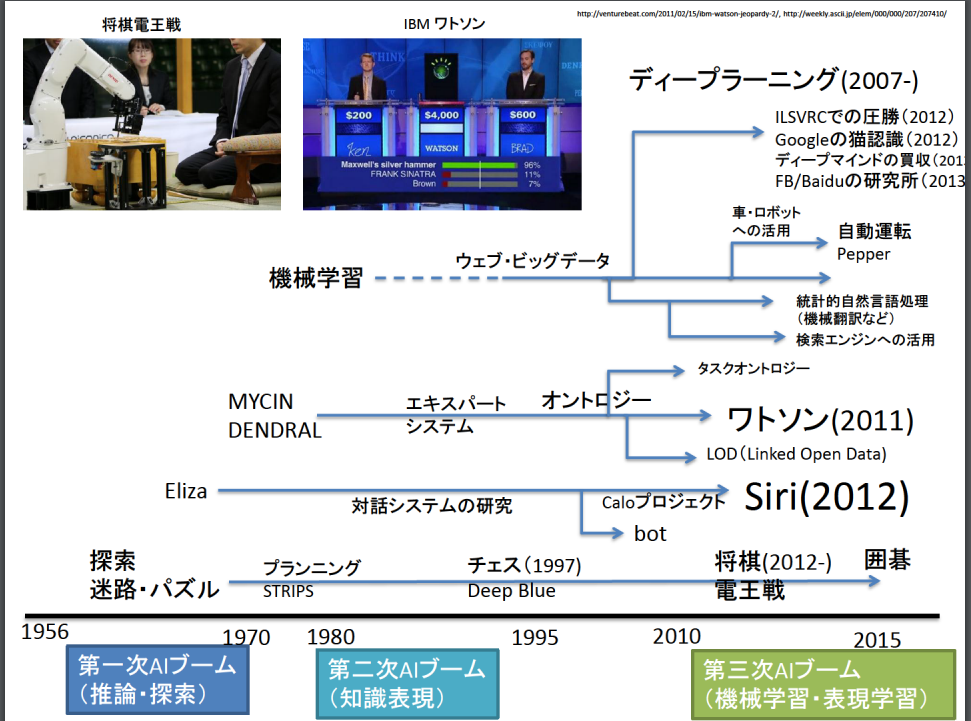
\includegraphics[scale=0.4, clip]{./img/AI_History.png}
        \caption{第一次AIブームから今までの流れ\newline(引用:https://bit.ly/2Wc9Ykb)}
        \label{fig:第一次AIブームから今までの流れ}
    \end{center}
\end{screen}
\end{figure}\\
スマートスピーカなどの対話型のAIがGoogleやAmazon,IBMによって商品化され,現在ではスマートフォンにもSiriというAIが搭載されるなどその存在は非常に身近になっており,その種類も非常に多岐にわたる.
\begin{figure}[!ht]
    \begin{screen}
    \begin{center}
        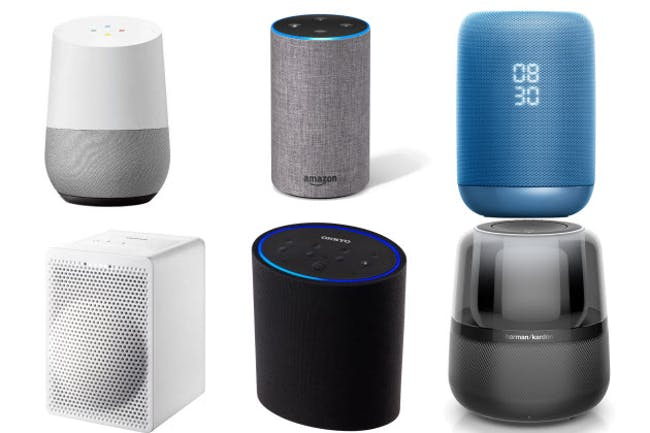
\includegraphics[scale=0.6, clip]{./img/smartspeaker_list.jpg}
        \caption{多種多様なスマートスピーカー}
        \label{fig:多種多様なスマートスピーカー}
    \end{center}
\end{screen}
\end{figure}\\
また囲碁や将棋,チェスなどの競技においても,プロにAIが勝利するなどその精度は以前から高いが,そのAIは一つの競技でしか使用できない特化型人工知能(AGI)でありった.
しかし,英DeepMindが発表したAlphaZeroという様々なボードゲームに対応できる汎用性を持ったAIが発表され,汎用人工知能(GAI)の成長も著しい.\\
自然言語処理を用いた芸術の分野では,2012年にスタートした人工知能を使って小説を生成するプロジェクトが「星新一賞」の第一審査を通過した.
また,絵画や音楽に関してもAIが作成した肖像画が米競売大手クリスティーズのオークションで43万2500ドル(約4900万円)で落札され,AIを用いて新しい作品を作るものが出回っている.\\
 このようにAIの発展は様々な分野においてその成果を上げており,今後は業務の効率化や補助だけにとどまらず,自動車の自動運転や医療の現場でも人間の手よりも高精度なものとして活躍することが期待されている.\\
本研究ではAIによる楽曲生成についての実証実験を行う.
Googole brainによって公開されているTensorflowのライブラリであるMagentaはAI Duetや
そのライブラリを用いて学習データやノード数による楽曲の生成結果の違いを比較,検証し,AIによる楽曲制作が有用なものか調査する.\\
\section{本論文の構成}
本論文の構成は以下の通りである.\\
第1章では本論文の背景と目的について述べている.\\
第2章では本論文で利用する理論について述べている.\\
第3章では実験内容について述べている.\\
第4章では楽曲制作について述べている.\\
第5章ではAIを用いた楽曲制作についての本研究の結論について述べている.\\